\documentclass[aspectratio=169,handout]{beamer}
\usepackage{will_handley_beamer}
\usepackage{title_page}

% Commands
% --------
% - \arxiv{arxiv number}
% - \arxiv{<number>}            arxiv.org/abs/<number>
% - \oldarxiv{<arxiv number>}   arxiv.org/<number>
% - \doi{<doi>}                 doi.org/<doi>
% - \xkcd{<number>}             xkcd.com/<number>
% - \email{<email>}             <<email>>
% - \tthref{<website>}          <website>
% - \av[dist]{<quantity>}       <quantity>_{dist}
% - \student{<name>}{<detail>}{<photo>}

% Talk details
% ------------
\title{Sampling methods for high energy physics \& particle astrophysics}
%\subtitle{<+subtitle+>}
\date{19\textsuperscript{th} August 2024}

\begin{document}

\begin{frame}
    \titlepage
\end{frame}

%\begin{frame}
%    \frametitle{The nature of sampling}
%    <++>
%\end{frame}
%
%\begin{frame}
%    \frametitle{Monte carlo integration}
%    <++>
%\end{frame}

\begin{frame}
    \begin{columns}
        \column{0.48\textwidth}
        \begin{block}{\textbf{MCMC}}
            \only<16>{
                \begin{itemize}
                    \item Single ``walker''
                    \item Explores posterior
                    \item Fast, if proposal matrix is tuned
                    \item Parameter estimation, suspiciousness calculation
                    \item Channel capacity optimised for generating posterior samples
                \end{itemize}
            }
        \end{block}
            \includegraphics<1|handout:0>[width=\textwidth,page=16]{figures/himmelblau.pdf}%
            \includegraphics<2|handout:0>[width=\textwidth,page=17]{figures/himmelblau.pdf}%
            \includegraphics<3|handout:0>[width=\textwidth,page=18]{figures/himmelblau.pdf}%
            \includegraphics<4|handout:0>[width=\textwidth,page=19]{figures/himmelblau.pdf}%
            \includegraphics<5|handout:0>[width=\textwidth,page=20]{figures/himmelblau.pdf}%
            \includegraphics<6-15|handout:0>[width=\textwidth,page=21]{figures/himmelblau.pdf}%
        \centerline{\includegraphics<16>[width=0.5\textwidth,page=19]{figures/himmelblau.pdf}}
        \column{0.48\textwidth}
        \begin{block}<7->{\textbf{Nested sampling}}
            \only<16>{
                \begin{itemize}
                    \item Ensemble of ``live points''
                    \item Scans from prior to peak of likelihood
                    \item Slower, no tuning required
                    \item Parameter estimation, model comparison, tension quantification
                    \item Channel capacity optimised for computing partition function
                \end{itemize}
            }
        \end{block}
            \includegraphics<7|handout:0>[width=\textwidth,page=1]{figures/himmelblau.pdf}%
            \includegraphics<8|handout:0>[width=\textwidth,page=2]{figures/himmelblau.pdf}%
            \includegraphics<9|handout:0>[width=\textwidth,page=3]{figures/himmelblau.pdf}%
            \includegraphics<10|handout:0>[width=\textwidth,page=4]{figures/himmelblau.pdf}%
            \includegraphics<11|handout:0>[width=\textwidth,page=5]{figures/himmelblau.pdf}%
            \includegraphics<12|handout:0>[width=\textwidth,page=6]{figures/himmelblau.pdf}%
            \includegraphics<13|handout:0>[width=\textwidth,page=7]{figures/himmelblau.pdf}%
            \includegraphics<14|handout:0>[width=\textwidth,page=8]{figures/himmelblau.pdf}%
            \includegraphics<15|handout:0>[width=\textwidth,page=15]{figures/himmelblau.pdf}%
        \centerline{\includegraphics<16>[width=0.5\textwidth,page=4]{figures/himmelblau.pdf}} 
    \end{columns}
\end{frame}

\begin{frame}
    \frametitle{Nested sampling: numerical Lebesgue integration}
    \begin{columns}
        \column{0.5\textwidth}
        \fbox{\parbox{\textwidth}{
                \begin{itemize}
                    \item[0.] Start with $N$ random samples over the space.
                    \item[i.] Delete outermost sample, and replace with a new random one at higher integrand value.
        \end{itemize}}}
        \vspace{-5pt}
        \begin{itemize}
            \item The ``live points'' steadily contract around the peak(s) of the function.
            \item Discarded ``dead points'' can be weighted to form posterior, prior, or anything in between.
            \item Estimates the \textbf{density of states} and \textbf{partition function} $\C[3]{\log \mathcal{Z}(\beta)}$.
            \item The evolving ensemble of live points allows:
                \begin{itemize}
                    \item implementations to self-tune,
                    \item exploration of multimodal functions,
                    \item global and local optimisation.
                \end{itemize}
        \end{itemize}
        \column{0.5\textwidth}
        \includegraphics<1|handout:0>[width=\textwidth,page=1]{figures/himmelblau}%
        \includegraphics<2|handout:0>[width=\textwidth,page=2]{figures/himmelblau}%
        \includegraphics<3|handout:0>[width=\textwidth,page=3]{figures/himmelblau}%
        \includegraphics<4|handout:0>[width=\textwidth,page=4]{figures/himmelblau}%
        \includegraphics<5|handout:0>[width=\textwidth,page=5]{figures/himmelblau}%
        \includegraphics<6|handout:0>[width=\textwidth,page=6]{figures/himmelblau}%
        \includegraphics<7|handout:0>[width=\textwidth,page=7]{figures/himmelblau}%
        \includegraphics<8|handout:0>[width=\textwidth,page=14]{figures/himmelblau}%
        \includegraphics<9->[width=\textwidth,page=15]{figures/himmelblau}%
    \end{columns}
\end{frame}

\begin{frame}
    \frametitle{The nested sampling zoo \hspace{170pt} \arxiv{2205.15570}}
    %\begin{columns}
    %    \begin{column}{0.33}
    %        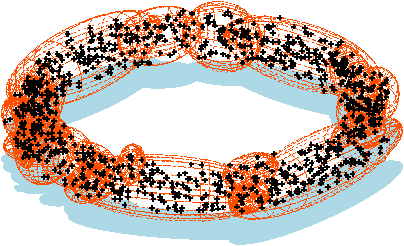
\includegraphics[width=\textwidth]{figures/multinest}
    %    \end{column} 
    %\end{columns}
    \begin{columns}[t]
        \column{0.3\textwidth}
        \texttt{MultiNest}~\arxiv{0809.3437}
        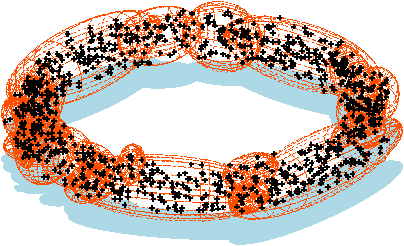
\includegraphics[width=\textwidth]{figures/multinest}
        \texttt{UltraNest}~\arxiv{2101.09604}
        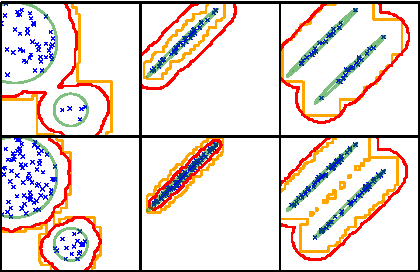
\includegraphics[width=\textwidth]{figures/radfriends}
        \texttt{nautilus}~\arxiv{2306.16923} 
        \column{0.4\textwidth}
        \texttt{PolyChord}~\arxiv{1506.00171}
        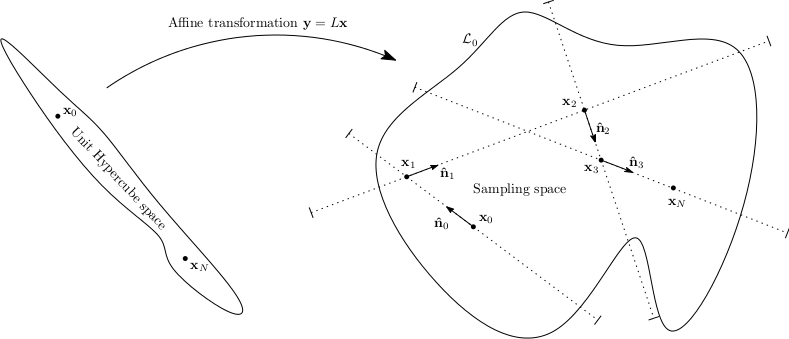
\includegraphics[width=\textwidth]{figures/polychord}
        \vfill
        \texttt{NeuralNest}~\arxiv{1903.10860}
        \begin{columns}
            \column{0.55\textwidth}
            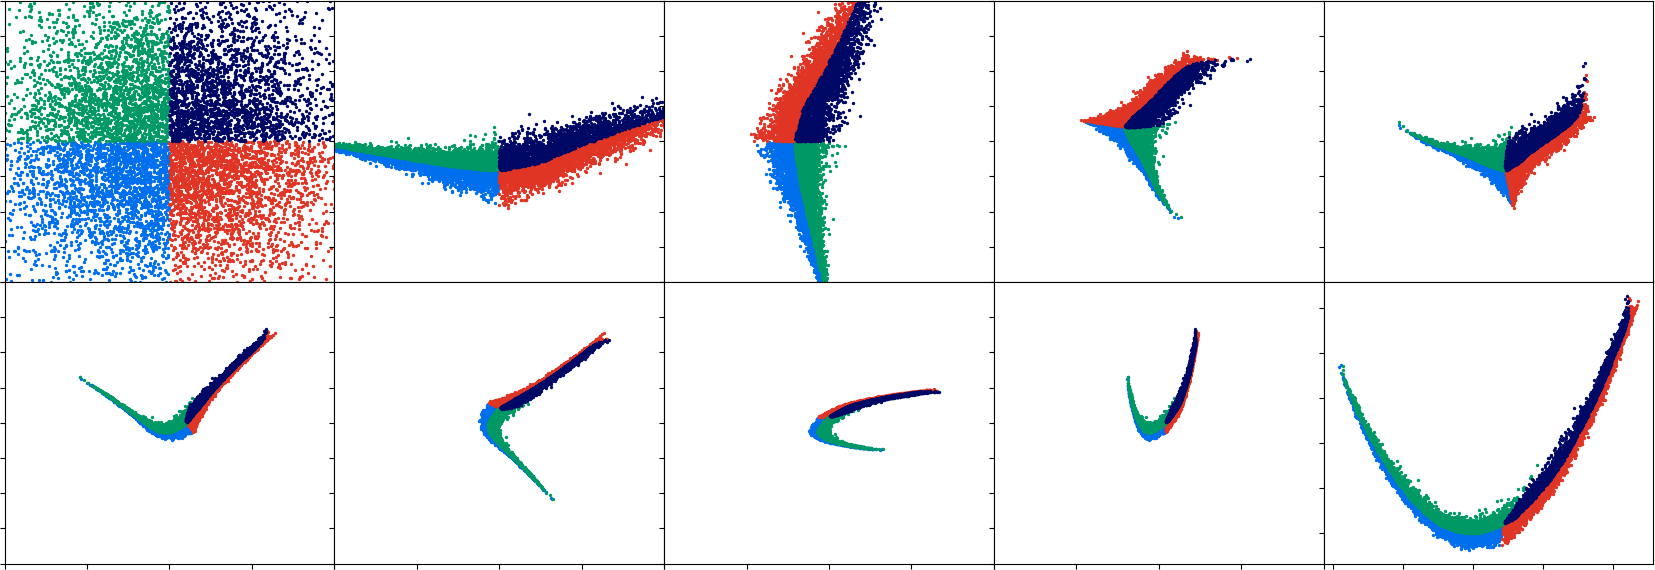
\includegraphics[width=\textwidth]{figures/rosenbrock_flow.png}
            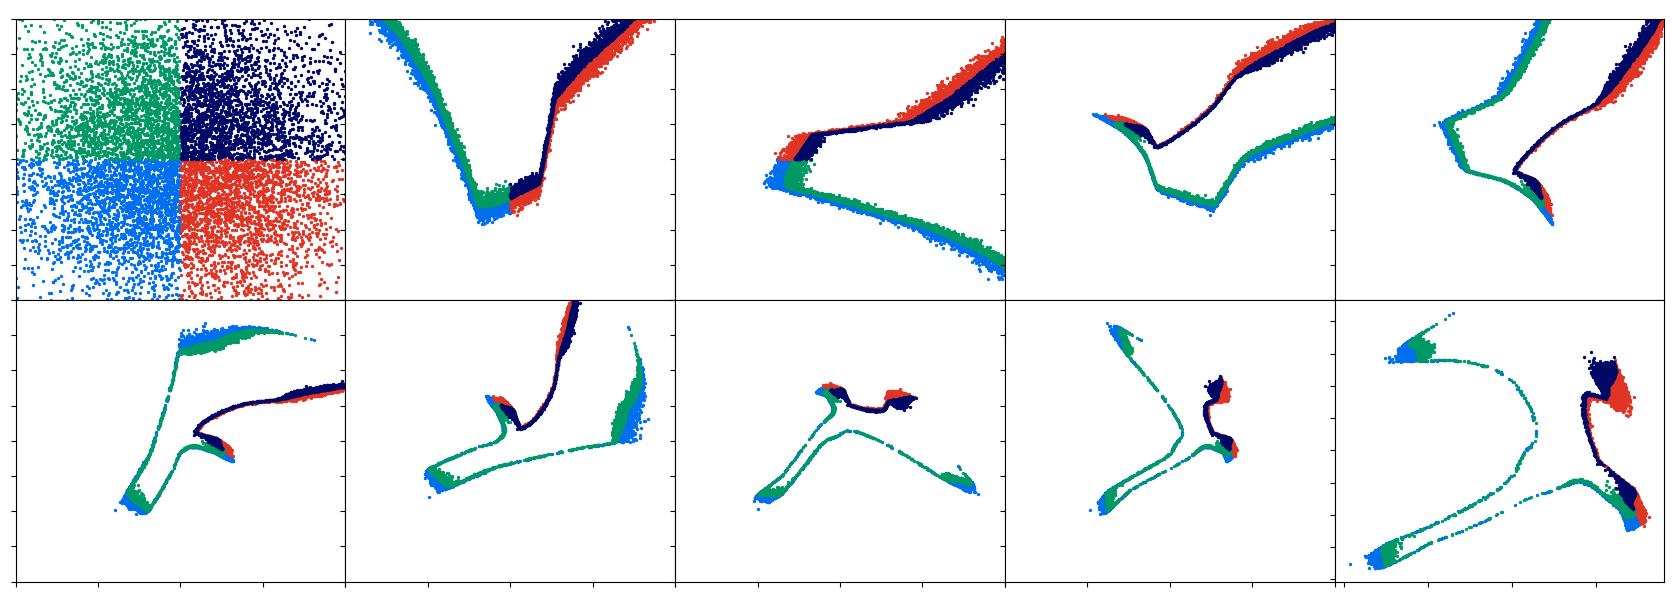
\includegraphics[width=\textwidth]{figures/himmelblau_flow.png}
            \column{0.45\textwidth}
            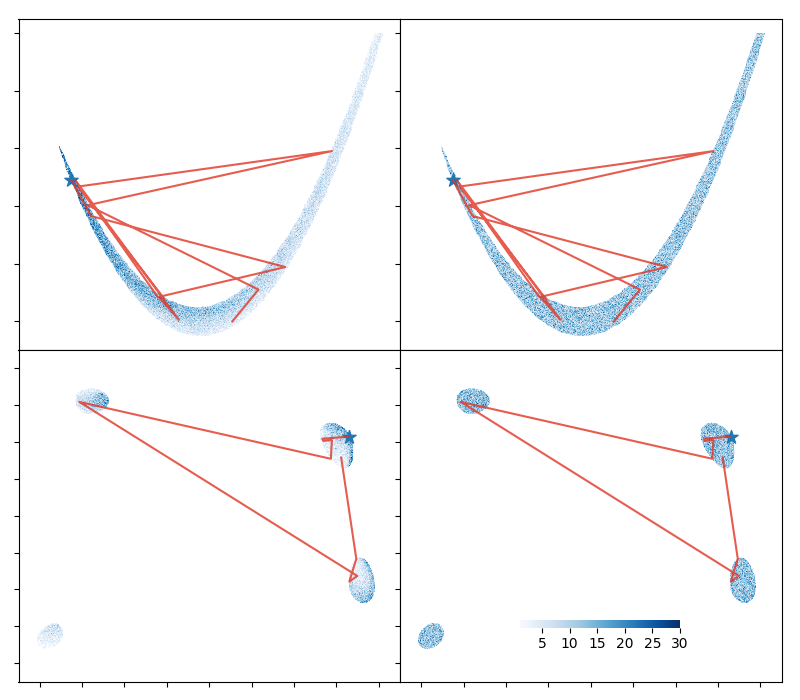
\includegraphics[width=\textwidth]{figures/chains.png}
        \end{columns}
        \texttt{nessai}~\arxiv{2102.11056} \texttt{nora}~\arxiv{2305.19267} \texttt{jaxnest}~\arxiv{2012.15286}
        \vfill
        \column{0.3\textwidth}
        \texttt{DNest}~\arxiv{1606.03757}
        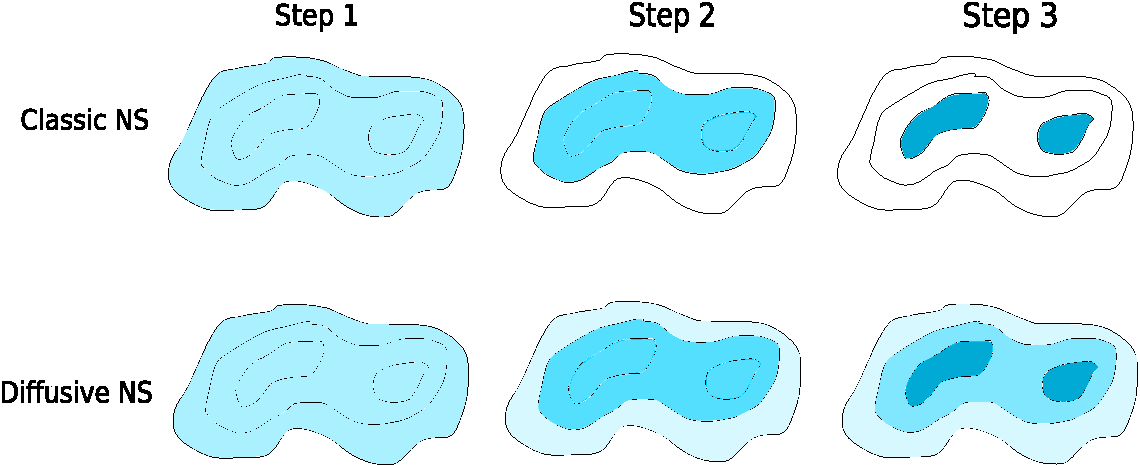
\includegraphics[width=\textwidth]{figures/dnest}
        \texttt{ProxNest}~\arxiv{2106.03646}
        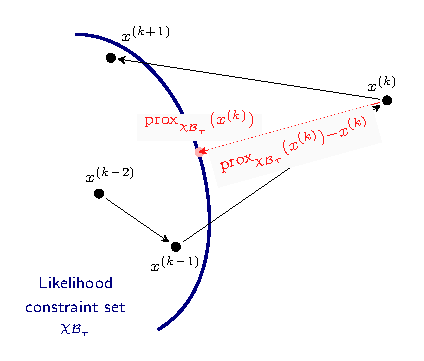
\includegraphics[width=\textwidth]{figures/proxnest_diagram}
        \texttt{dynesty}~\arxiv{1904.02180} 
        \vfill
    \end{columns}
\end{frame}

\begin{frame}
    \frametitle{Lattice field theory}
    \framesubtitle{Applications of nested sampling}
\student{david_yallup}{David Yallup}{PDRA}
    \begin{columns}
        \column{0.5\textwidth}
        \begin{itemize}
            \item Consider standard field theory Lagrangian:
                \[ Z(\beta) = \int D\phi e^{-\beta S(\phi)}, \quad S(\phi) = \int dx^\mu \mathcal{L}(\phi) \]
            \item Discretize onto spacetime grid.
            \item Compute partition function
            \item NS unique traits:
                \begin{itemize}
                    \item Get full partition function for free
                    \item allows for critical tuning
                    \item avoids critical slowing down
                \end{itemize}
            \item Applications in lattice gravity, QCD, condensed matter physics
        \end{itemize}
        \column{0.5\textwidth}
        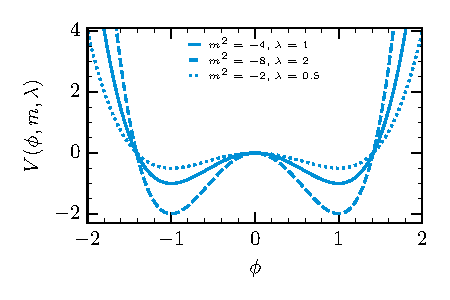
\includegraphics[width=0.49\textwidth]{figures/potential_shape}
        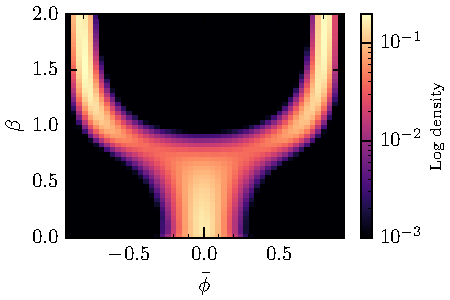
\includegraphics[width=0.49\textwidth]{figures/2d_phase}
        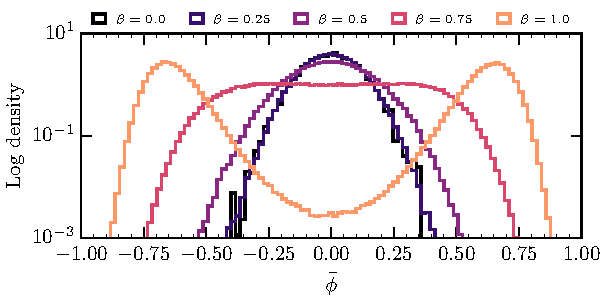
\includegraphics[width=\textwidth]{figures/lattice_field_theory.pdf}
    \end{columns}
\end{frame}

\begin{frame}
    \frametitle{Fast estimation of small $p$-values~\arxiv{2106.02056}(PRL)}
    \framesubtitle{Applications of nested sampling}
    \student{andrew_fowlie}{Andrew Fowlie}{}
    \begin{columns}
        \column{0.55\textwidth}
        \begin{itemize}
            \item Nested sampling for frequentist computation!?
            \item $p$-value: $P(\lambda>\lambda^*|H_0)$ -- probability that test statistic $\lambda$ is at least as great as observed $\lambda^*$.
            \item Computation of a tail probability from sampling distribution of $\lambda$ under $H_0$.
            \item For gold-standard $5\sigma$, this is very expensive to simulate directly ($\sim10^9$ by definition).
            \item Need insight/approximation to make efficient.
            \item Nested sampling is tailor-made for this, just make switch: $X\leftrightarrow p$, $\mathcal{L}\leftrightarrow\lambda$, $\theta \leftrightarrow x$.
            \item The only real conceptual shift is switching the integrator from parameter- to data-space.
        \end{itemize}
        \column{0.45\textwidth}
        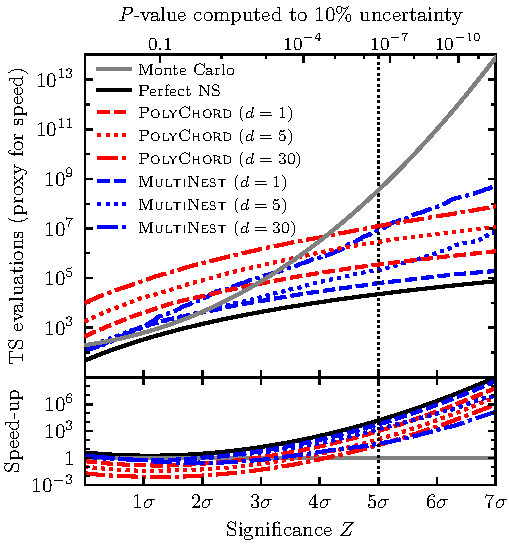
\includegraphics[width=\textwidth]{figures/pvalue.pdf}
    \end{columns}
\end{frame}

\begin{frame}
    \frametitle{Cross section calculation}
    \framesubtitle{Applications of nested sampling}
    \student{david_yallup}{David Yallup}{PDRA}
    \begin{columns}
        \column{0.56\textwidth}
        \begin{columns}
            \column{0.67\textwidth}
            \begin{itemize}
                \item Nested sampling for cross section computation/event generation
            \end{itemize}
            \column{0.3\textwidth}
            \[\sigma = \int_\Omega d\Phi |\mathcal{M}|^2.\]
        \end{columns}
        \begin{itemize}
            \item Nested sampling can explore the phase space $\Omega$ and compute integral blind with comparable efficiency to HAAG/RAMBO~\arxiv{2205.02030}.
            \item Bayesian sparse reconstruction~\arxiv{1809.04598} applied to bump hunting allows evidence-based detection of signals in phenomenological backgrounds~\arxiv{2211.10391}.
            \item Fine tuning quantification
        \end{itemize}
        \column{0.17\textwidth}
        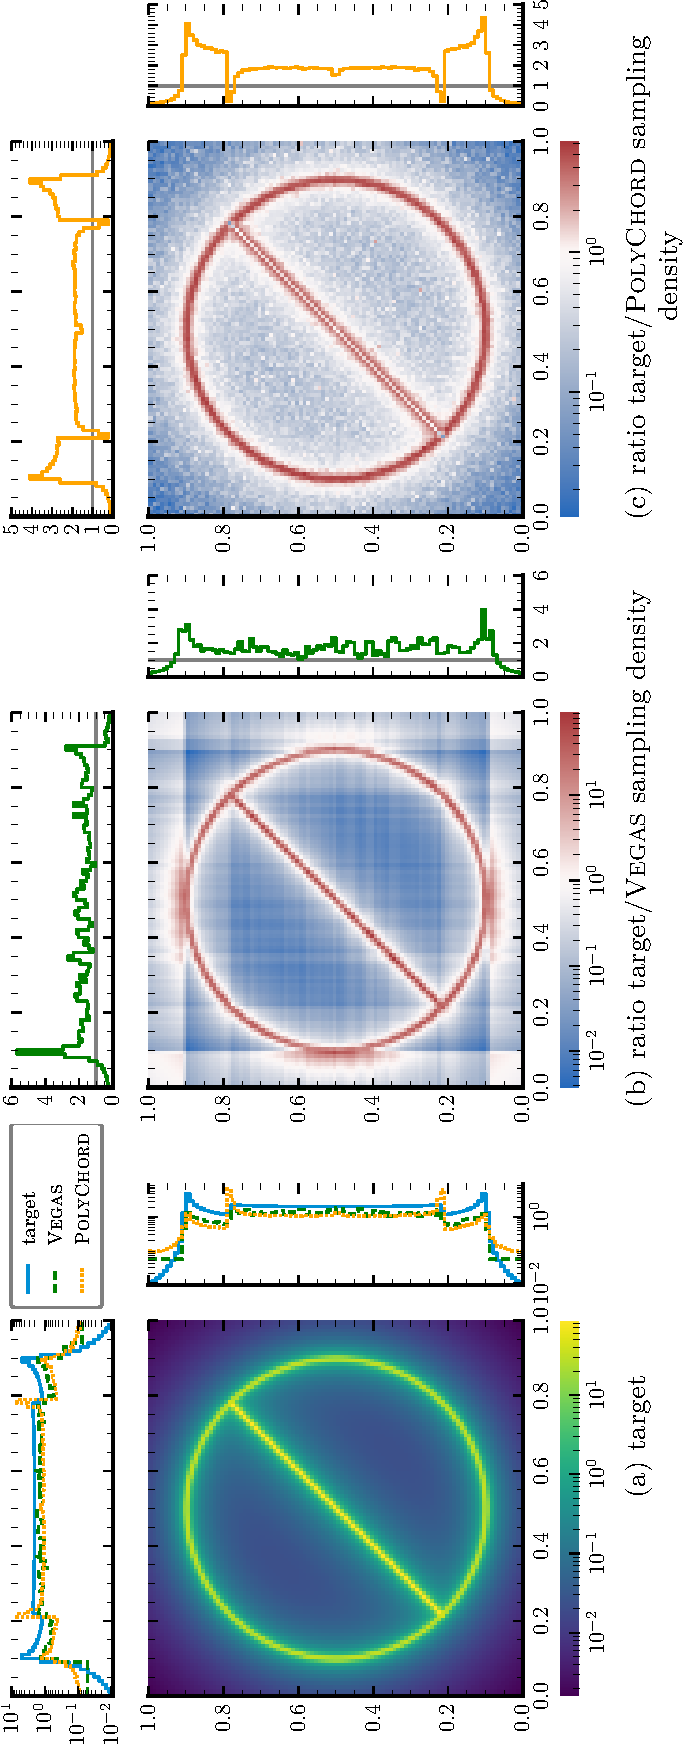
\includegraphics[width=\textwidth]{figures/phase_space_1-pdfjam-crop.pdf}
        \column{0.27\textwidth}
        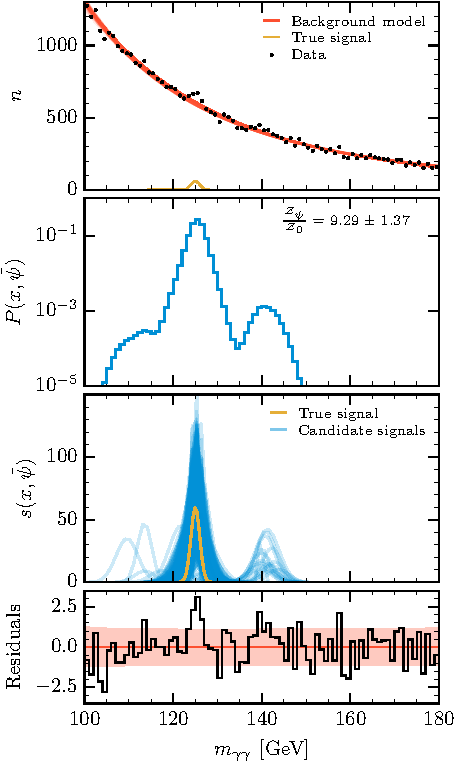
\includegraphics[width=\textwidth]{figures/psi_predict-crop.pdf}
    \end{columns}
\end{frame}

\begin{frame}
    \frametitle{Quantification of fine tuning~\arxiv{2101.00428}~\arxiv{2205.13549}}
    \framesubtitle{Applications of nested sampling}
    \student{gambit}{GAMBIT}{dm-cosmo WG}
    \vspace{8pt}
    \begin{columns}
        \column{0.55\textwidth}
        \begin{itemize}
            \item Example: Cosmological constraints on decaying axion-like particles~\arxiv{2205.13549}.
            %\item Subset of parameters $\xi,m_a,\tau,g_{a\gamma}$: ALP fraction, mass, lifetime and photon coupling.
                {(\small Also vary cosmology, $\tau_n$ and nuisance params)}
            \item Data: CMB, BBN, FIRAS, SMM, BAO.
            \item Standard profile likelihood fit shows ruled out regions and best-fit point.
            \item<2-> Nested sampling scan:
                \begin{itemize}
                    \item Quantifies amount of parameter space ruled out with Kullback-Liebler divergence $\mathcal{D}_\mathrm{KL}$.
                    \item Identifies best fit region as statistically irrelevant from information theory/Bayesian.
                    \item No evidence for decaying ALPs. Fit the data equally well: but more constrained parameters create Occam penalty.
                \end{itemize}
        \end{itemize}
        \column{0.45\textwidth}
        \includegraphics<1|handout:0>[width=\textwidth]{figures/ALP_1.pdf}
        \includegraphics<2          >[width=\textwidth]{figures/ALP_2.pdf}
        \includegraphics<3|handout:0>[width=\textwidth]{figures/ALP_3.pdf}
    \end{columns}
    
\end{frame}


%\begin{frame}
%    \frametitle{GAMBIT}
%    <++>
%\end{frame}

\begin{frame}
    \frametitle{Model comparison $\C[3]{\mathcal{Z}=P(D|M)}$}
    \begin{itemize}
        \item Bayesian model comparison allows mathematical derivation of key philosophical principles.
    \end{itemize}
    \begin{columns}[t]
        \column{0.47\textwidth}
        Viewed from data-space $D$:
        \begin{block}{Popper's falsificationism}
            \begin{itemize}
                \item Prefer models that make bold predictions.
                \item if proven true, model more likely correct.
            \end{itemize}
        \end{block}
        \includegraphics<1|handout:0>[width=\textwidth, page=1]{figures/popper}%
        \includegraphics<2|handout:0>[width=\textwidth, page=2]{figures/popper}%
        \includegraphics<3>[width=\textwidth, page=3]{figures/popper}%
        \begin{itemize}
            \item Falsificationism comes from normalisation
        \end{itemize}
        \column{0.47\textwidth}
        Viewed from parameter-space $\theta$:
        \begin{block}{Occam's razor}
            \begin{itemize}
                \item Models should be as simple as possible
                \item \ldots but no simpler
            \end{itemize}
        \end{block}
        \begin{itemize}
            \item Occam's razor equation:
                \[\C[3]{\log\mathcal{Z}} = \av[{\C[0]{\mathcal{P}}}]{\C[2]{\log\mathcal{L}}} - \mathcal{D}_\text{KL}\]
            \item ``Occam penalty'': KL divergence between \C[1]{prior~$\pi$} and \C[0]{posterior~$\mathcal{P}$}.
                \[ \mathcal{D}_\text{KL}\sim \log\frac{\text{\C[1]{Prior volume} }}{\text{\C[0]{Posterior volume}}}\]
        \end{itemize}
    \end{columns}
\end{frame}

\begin{frame}
    \frametitle{Conclusions}
    \framesubtitle{\tthref{github.com/handley-lab}}
    \tikz[overlay,remember picture]
        \node[anchor=north east] (A) at ($(current page.north east)+(0,0)$) {
        
\includegraphics[width=0.09\textheight]{figures/students/adam_ormondroyd.jpg}%
        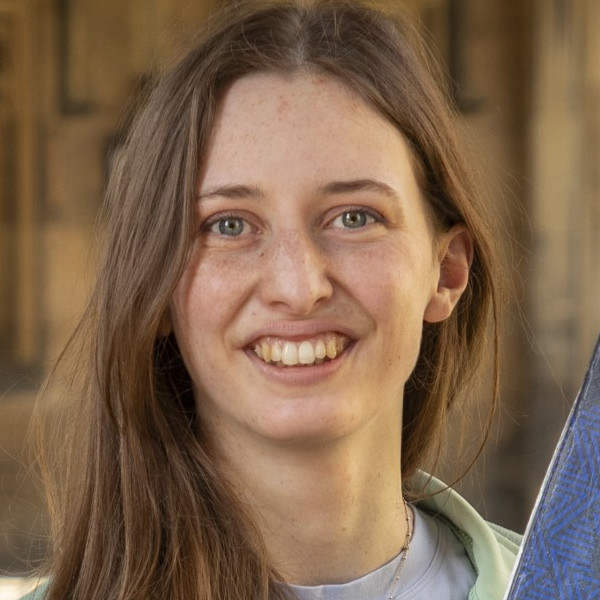
\includegraphics[width=0.09\textheight]{figures/students/charlotte_priestley.jpg}%
        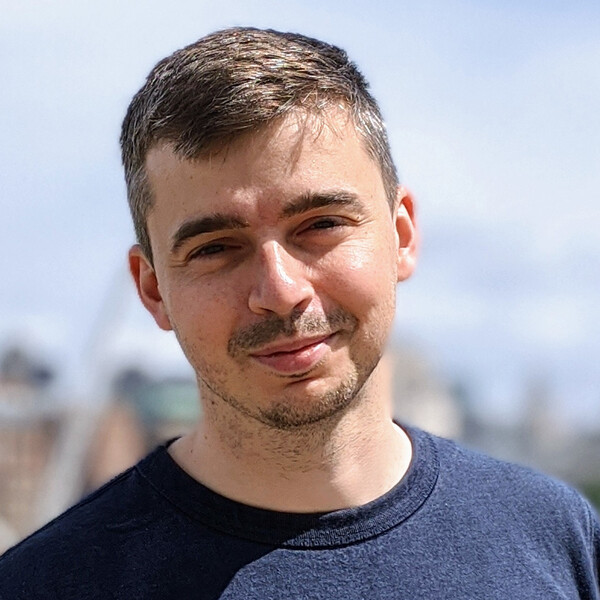
\includegraphics[width=0.09\textheight]{figures/students/david_yallup.jpg}%
        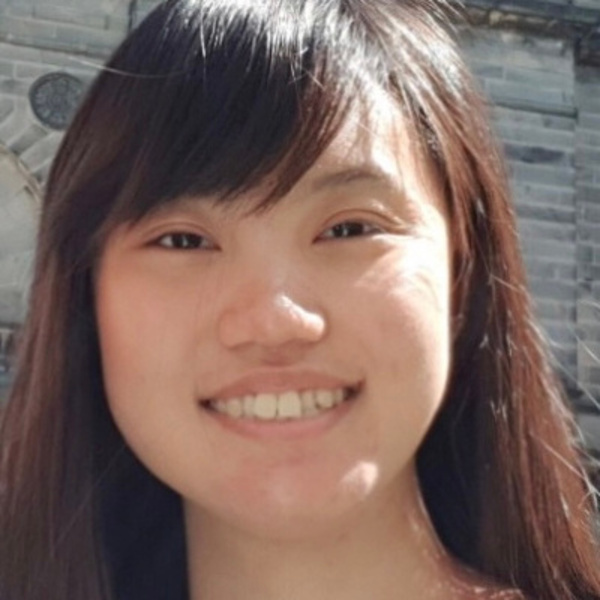
\includegraphics[width=0.09\textheight]{figures/students/dily_ong.jpg}%
        
\includegraphics[width=0.09\textheight]{figures/students/george_carter.jpg}%
        
\includegraphics[width=0.09\textheight]{figures/students/harry_bevins.jpg}%
        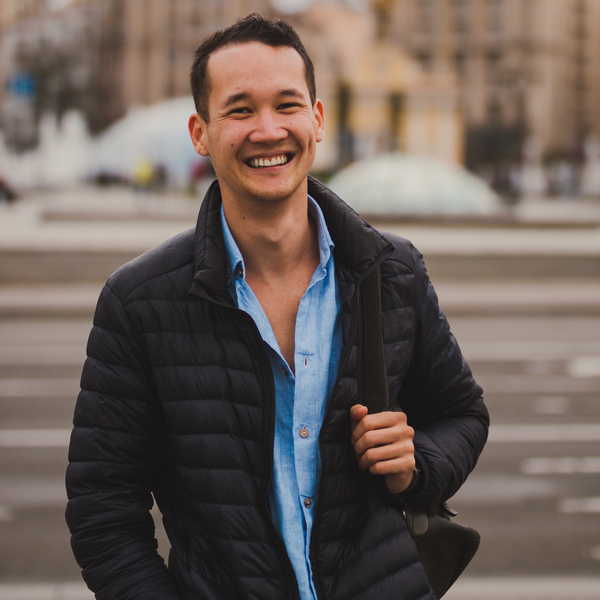
\includegraphics[width=0.09\textheight]{figures/students/kilian_scheutwinkel.jpg}%
        
\includegraphics[width=0.09\textheight]{figures/students/metha_prathaban.jpg}%
        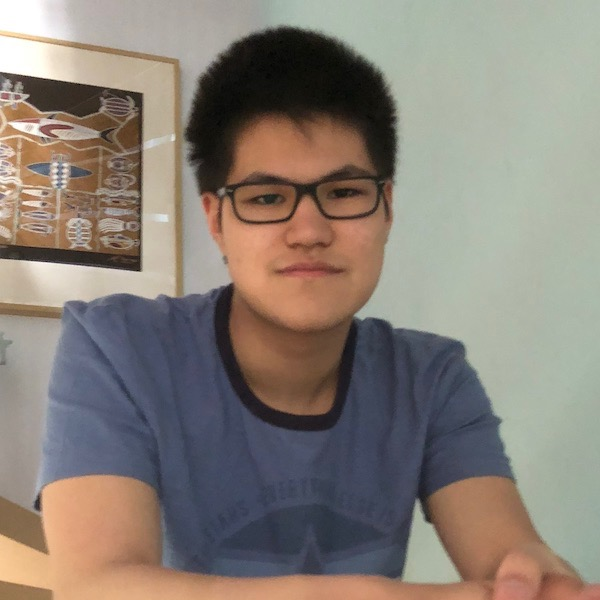
\includegraphics[width=0.09\textheight]{figures/students/namu_kroupa.jpg}%
        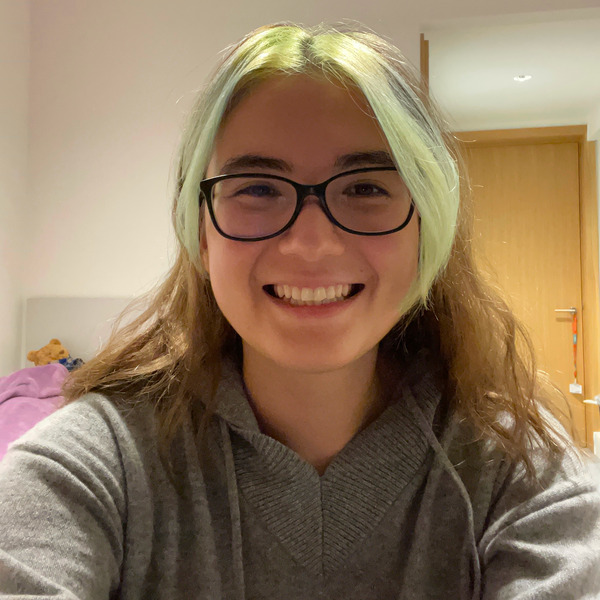
\includegraphics[width=0.09\textheight]{figures/students/sinah_legner.jpg}%
        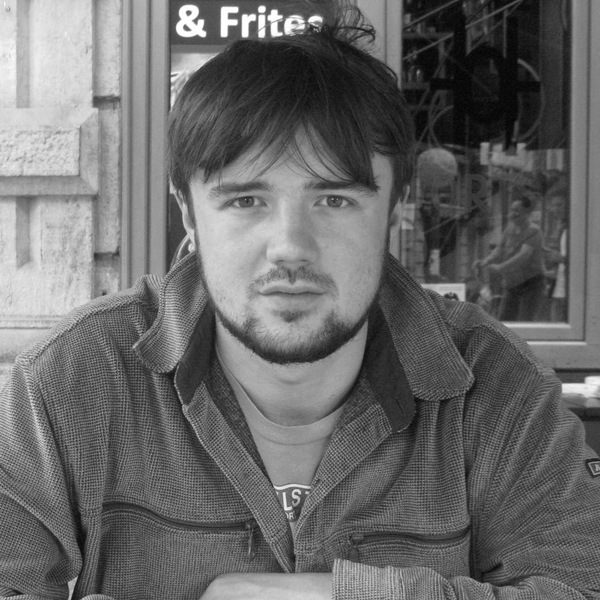
\includegraphics[width=0.09\textheight]{figures/students/sam_leeney.jpg}%
        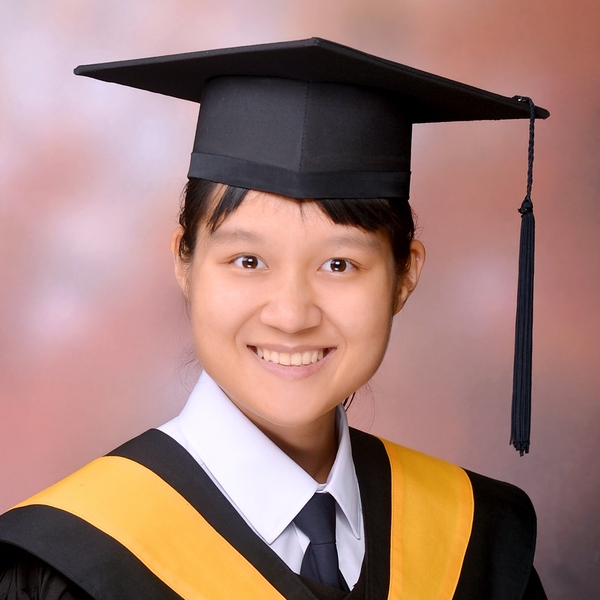
\includegraphics[width=0.09\textheight]{figures/students/wei-ning_deng.jpg}%
    };
    \vspace{-0.1\textheight}
    \begin{columns}
        \column{0.65\textwidth}
    \begin{itemize}
        \item Nested sampling is a multi-purpose numerical tool for:
            \begin{itemize}
                \item Numerical integration $\int f(x) dV$,
                \item Exploring/scanning/optimising \textit{a priori} unknown functions,
                \item Performing Bayesian inference and model comparison.
            \end{itemize}
        \item It is applied widely across cosmology \& particle physics.
        \item It's unique traits as the only numerical Lebesgue integrator mean with compute it will continue to grow in importance.
    \end{itemize}
        \column{0.35\textwidth}
    %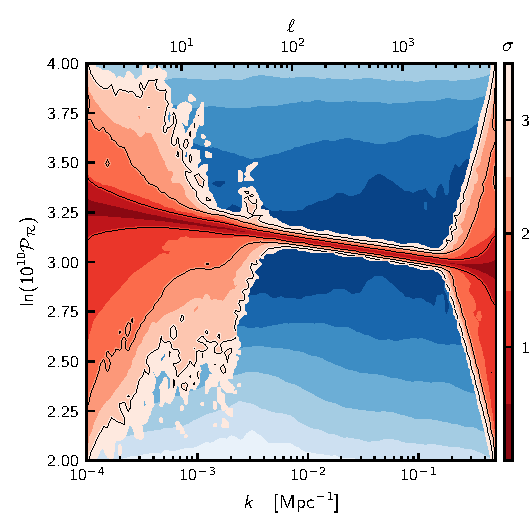
\includegraphics[height=0.6\textwidth]{figures/pps_both}%
    %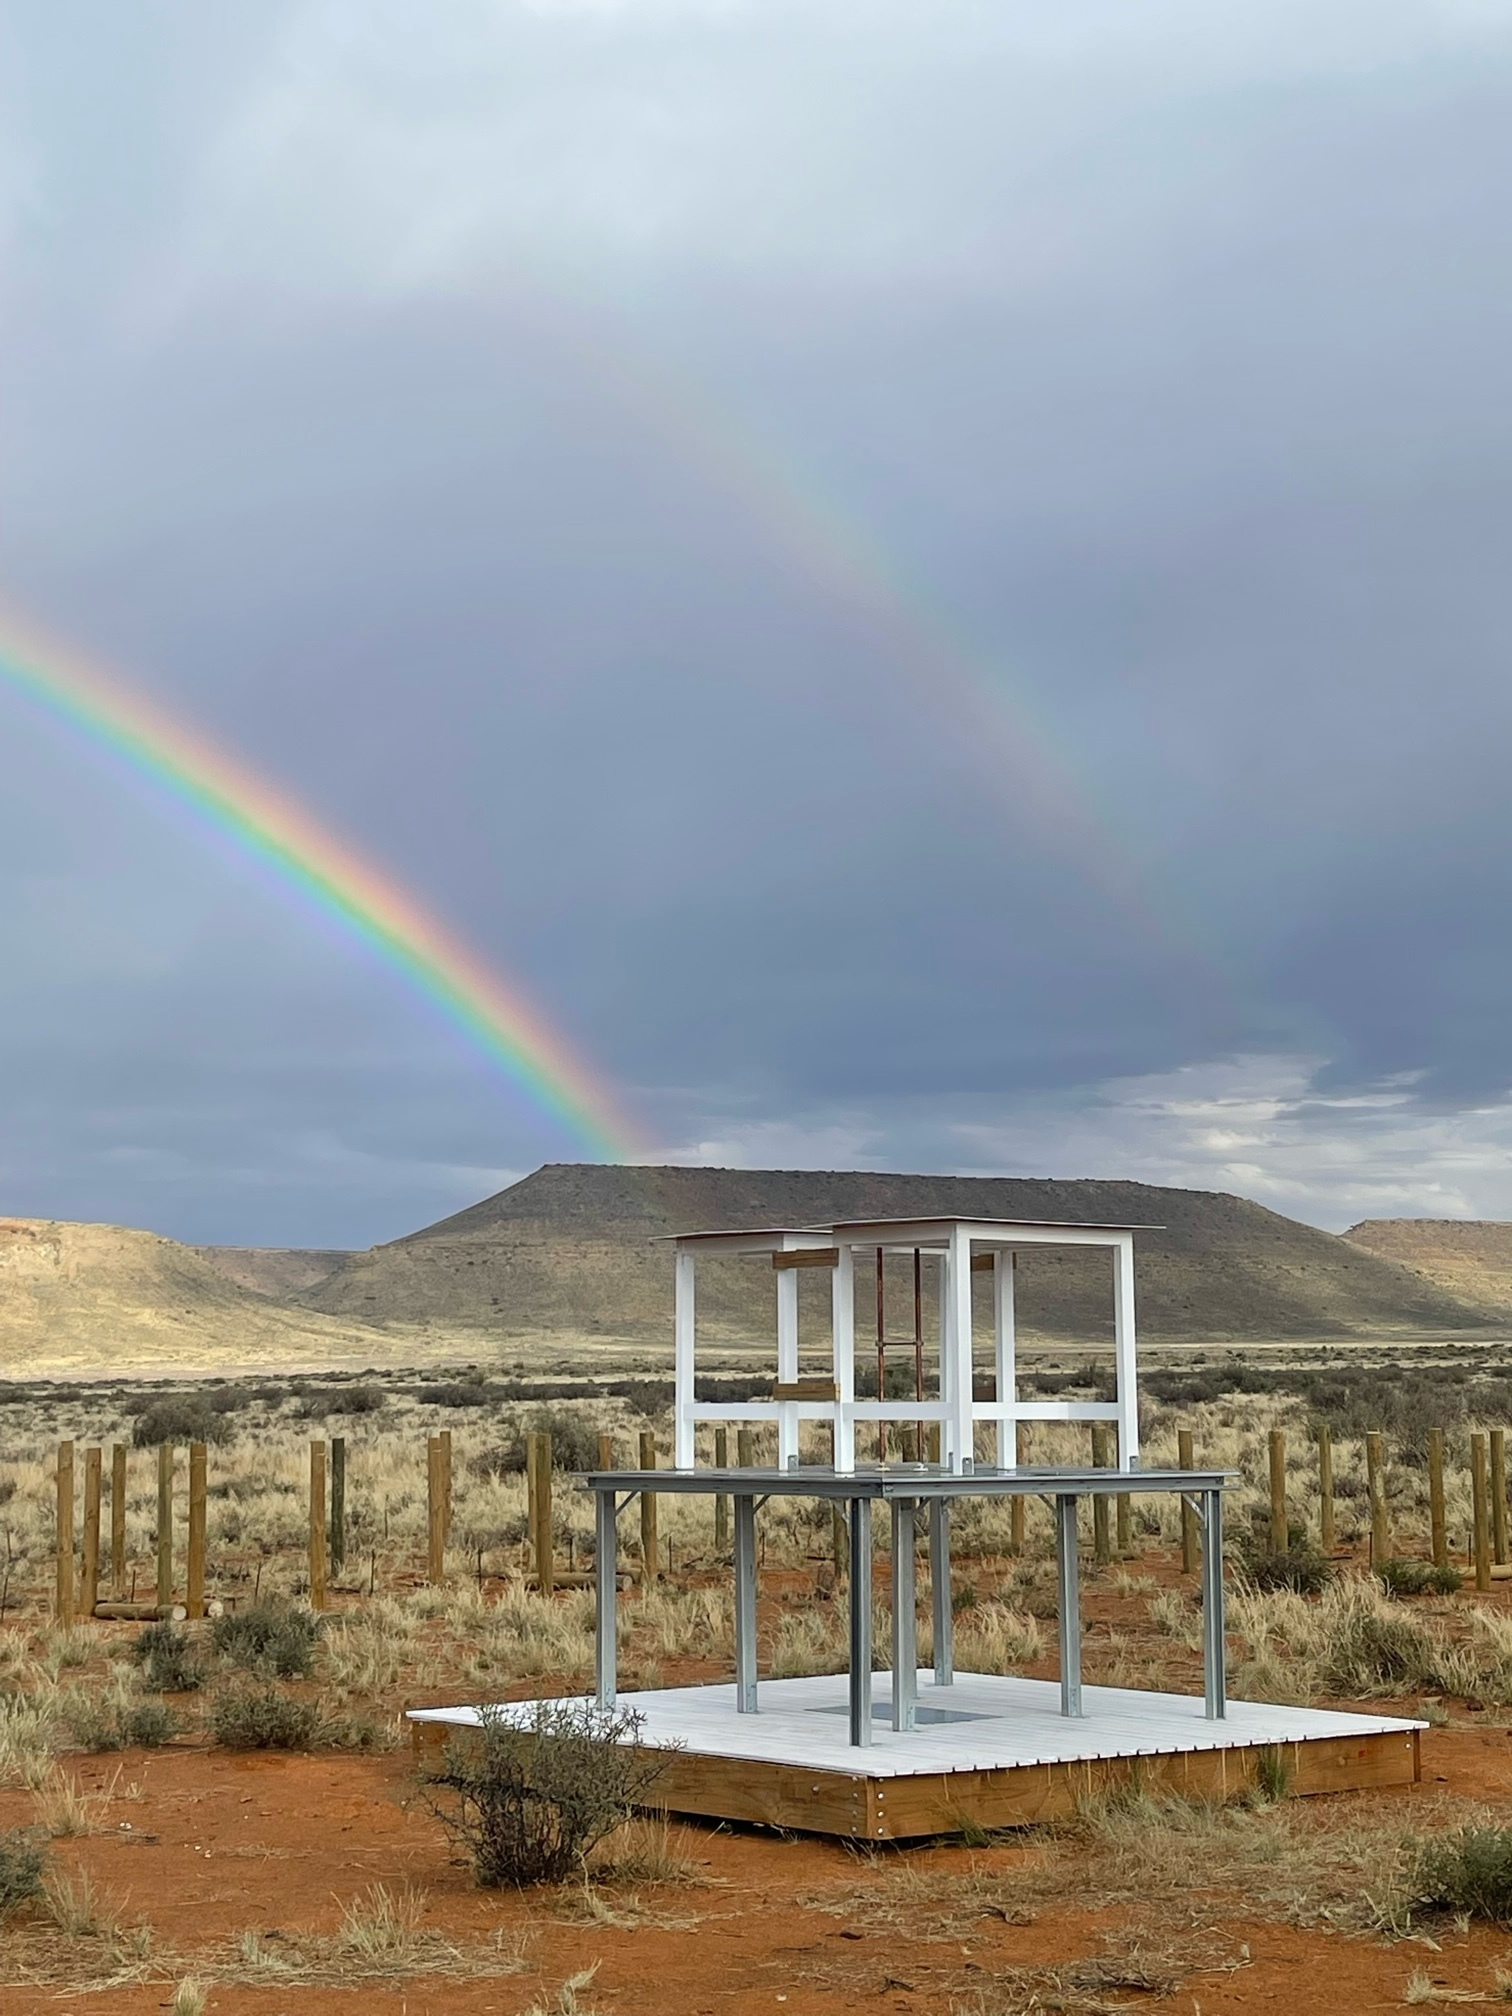
\includegraphics[height=0.6\textwidth]{figures/REACH_2}%
    \end{columns}
    %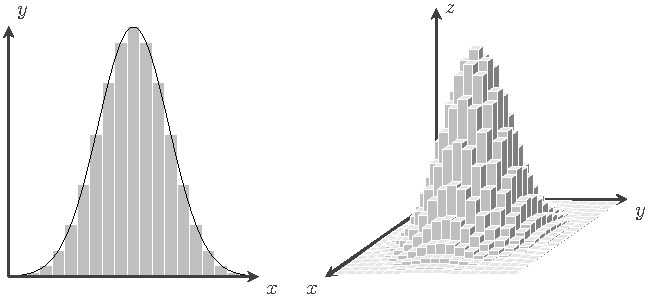
\includegraphics[height=0.2\textwidth]{figures/integration}%
    %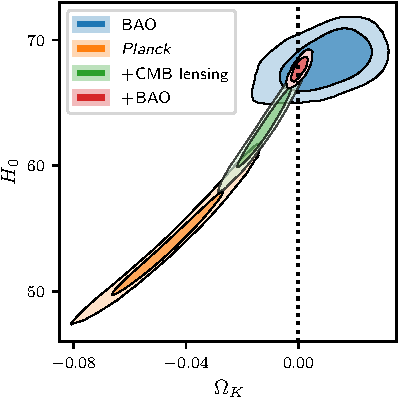
\includegraphics[height=0.2\textwidth]{figures/curvature_3}%
    %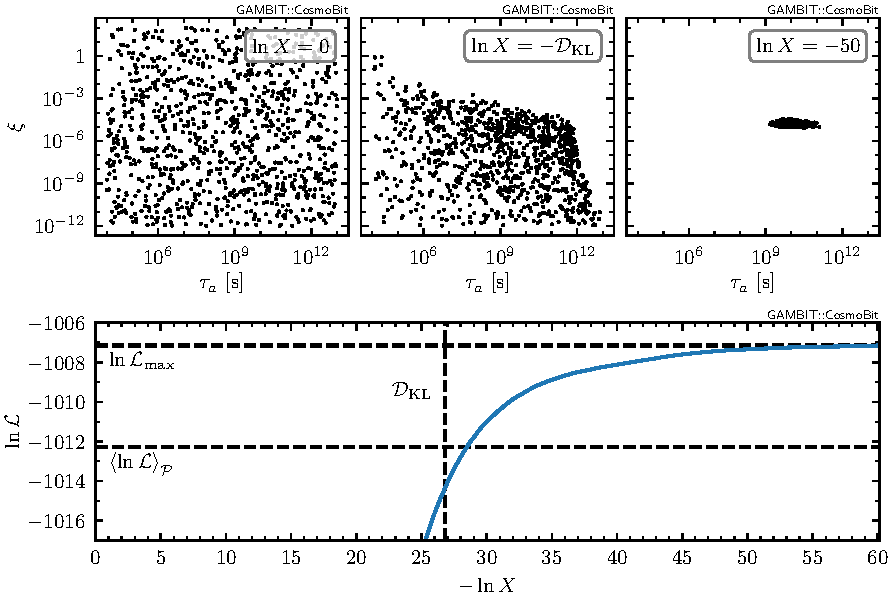
\includegraphics[height=0.2\textwidth]{figures/ALP_3}%
\end{frame}

\end{document}
